%% LyX 2.3.3 created this file.  For more info, see http://www.lyx.org/.
%% Do not edit unless you really know what you are doing.
\documentclass[12pt,english]{article}
\usepackage[osf]{mathpazo}
\renewcommand{\sfdefault}{lmss}
\renewcommand{\ttdefault}{lmtt}
\usepackage[T1]{fontenc}
\usepackage[latin9]{inputenc}
\usepackage[paperwidth=30cm,paperheight=35cm]{geometry}
\geometry{verbose,tmargin=2cm,bmargin=2cm}
\setlength{\parindent}{0bp}
\usepackage{amsmath}
\usepackage{amssymb}

\makeatletter
\@ifundefined{date}{}{\date{}}
%%%%%%%%%%%%%%%%%%%%%%%%%%%%%% User specified LaTeX commands.
\usepackage{tikz}
\usetikzlibrary{matrix,arrows,decorations.pathmorphing}
\usetikzlibrary{shapes.geometric}
\usepackage{tikz-cd}
\usepackage{amsthm}
\usepackage{xparse,etoolbox}

\theoremstyle{plain}
\newtheorem{theorem}{Theorem}[section]
\newtheorem{lemma}[theorem]{Lemma}
\newtheorem{prop}{Proposition}[section]
\newtheorem*{cor}{Corollary}
\theoremstyle{definition}
\newtheorem{defn}{Definition}[section]
\newtheorem{ex}{Exercise} 
\newtheorem{example}{Example}[section]
\theoremstyle{remark}
\newtheorem*{rem}{Remark}
\newtheorem*{note}{Note}
\newtheorem{case}{Case}
\usepackage{graphicx}
\usepackage{amssymb}
\usepackage{tikz-cd}
\usetikzlibrary{calc,arrows,decorations.pathreplacing}
\tikzset{mydot/.style={circle,fill,inner sep=1.5pt},
commutative diagrams/.cd,
  arrow style=tikz,
  diagrams={>=latex},
}

\usepackage{babel}
\usepackage{hyperref}
\hypersetup{
    colorlinks,
    citecolor=blue,
    filecolor=blue,
    linkcolor=blue,
    urlcolor=blue
}
\usepackage{pgfplots}
\usetikzlibrary{decorations.markings}
\pgfplotsset{compat=1.9}


\newcommand{\blocktheorem}[1]{%
  \csletcs{old#1}{#1}% Store \begin
  \csletcs{endold#1}{end#1}% Store \end
  \RenewDocumentEnvironment{#1}{o}
    {\par\addvspace{1.5ex}
     \noindent\begin{minipage}{\textwidth}
     \IfNoValueTF{##1}
       {\csuse{old#1}}
       {\csuse{old#1}[##1]}}
    {\csuse{endold#1}
     \end{minipage}
     \par\addvspace{1.5ex}}
}

\raggedbottom

\blocktheorem{theorem}% Make theo into a block
\blocktheorem{defn}% Make defi into a block
\blocktheorem{lemma}% Make lem into a block
\blocktheorem{rem}% Make rem into a block
\blocktheorem{cor}% Make col into a block
\blocktheorem{prop}% Make prop into a block


\usepackage[bottom]{footmisc}

\makeatother

\usepackage{babel}
\begin{document}
\title{Linear Analysis Homework 10}
\author{Michael Nelson}
\maketitle

\section*{Problem 1}

\begin{prop}\label{prop} Let $\|\cdot\|_{\infty}\colon C[a,b]\times C[a,b]\to\mathbb{R}$
be given by
\begin{equation}
\|f\|_{\infty}=\sup\{|f(x)|\mid x\in[a,b]\}\label{eq:supnorm}
\end{equation}
for all $f\in C[a,b]$. Then $\|\cdot\|_{\infty}$ is a norm. Moreover,
the pair $(C[a,b],\|\cdot\|_{\infty})$ forms a Banach space. \end{prop}

\begin{proof} Let us first show $\|\cdot\|_{\infty}$ is a norm.
First note that the set $\{|f(x)|\mid x\in[a,b]\}$ is non-empty and
bounded above (since $f$ is continuous on a compact interval and
hence attains a maximum). Therefore the supremum (\ref{eq:supnorm})
exists. 

~~~For positive-definiteness, let $f\in C[a,b]$. Then
\begin{align*}
\|f\|_{\infty} & =\sup\{|f(x)|\mid x\in[a,b]\}\\
 & \geq\sup\{0\mid x\in[a,b]\}\\
 & =0.
\end{align*}
We have equality if and only if $|f(x)|=0$ for all $x\in[a,b]$,
and since $|\cdot|$ is positive-definite, this is equivalent to $f$
being the zero function.

~~~For absolute-homogeneity, let $f\in C[a,b]$ and $\alpha\in\mathbb{C}$.
Then 
\begin{align*}
\|\alpha f\|_{\infty} & =\sup\{|\alpha f(x)|\mid x\in[a,b]\}\\
 & =\sup\{|\alpha||f(x)|\mid x\in[a,b]\}\\
 & =|\alpha|\sup\{|f(x)|\mid x\in[a,b]\}\\
 & =|\alpha|\|f\|_{\infty},
\end{align*}
where the equality at the third line is justified by Proposition~(\ref{propsuplinearpositive})
(stated and proved in the Appendix).

~~~For subadditivity, let $f,g\in C[a,b]$. Then
\begin{align*}
\|f+g\|_{\infty} & =\sup\{|f(x)+g(x)|\mid x\in[a,b]\}\\
 & \leq\sup\{|f(x)|+|g(x)|\mid x\in[a,b]\}\\
 & =\sup\{|f(x)|\mid x\in[a,b]\}+\sup\{|g(x)|\mid x\in[a,b]\}\\
 & =\|f\|_{\infty}+\|g\|_{\infty},
\end{align*}
where the equality at the third line is justified by Proposition~(\ref{propsuplinearpositive2})
(stated and proved in the Appendix).

~~~Finally, to show that $(C[a,b],\|\cdot\|_{\infty})$ forms a
Banach space, we need to show that every Cauchy sequence in $(C[a,b],\|\cdot\|_{\infty})$
is convegent. Throughout the rest of the proof, we drop the notation
$(C[a,b],\|\cdot\|_{\infty})$ and simply write $C[a,b]$ instead.
Let $(f_{n})$ be a Cauchy sequence in $C[a,b]$. We first make the
observation that for each $x\in[a,b]$, the sequence $(f_{n}(x))$
forms a Cauchy sequence of complex numbers. Indeed, let $\varepsilon>0$.
Choose $N\in\mathbb{N}$ such that $m,n\geq N$ implies $\|f_{n}-f_{m}\|_{\infty}<\varepsilon$.
In other words, $m,n\geq N$ implies
\[
\sup\{|f_{n}(x)-f_{m}(x)|\mid x\in[a,b]\}<\varepsilon.
\]
In particular $m,n\geq N$ implies
\begin{equation}
|f_{n}(x)-f_{m}(x)|<\varepsilon\label{eq:mtoinf}
\end{equation}
for all $x\in[a,b]$. This proves our claim. 

~~~Since $\mathbb{C}$ is complete, we are justified in defining
$f\colon[a,b]\to\mathbb{C}$ by
\[
f(x):=\lim_{n\to\infty}f_{n}(x)
\]
for all $x\in[a,b]$. By taking $m\to\infty$ in (\ref{eq:mtoinf}),
we see that $(f_{n})$ converges \emph{uniformly }to $f$. In particular,
this implies $f$ is continuous (by the usual $\varepsilon/3$ trick).
Thus $f\in C[a,b]$. Finally, we note that convergence in $\|\cdot\|_{\infty}$
is equivalent to uniform convergence. Thus the Cauchy sequence $(f_{n})$
converges in the $\|\cdot\|_{\infty}$ norm to $f$. \end{proof}

\section*{Problem 2}

\begin{prop}\label{prop} Let $(V,\|\cdot\|)$ be a normed linear
space over $\mathbb{C}$ which satisfies the parallelogram law. Then
the map $\langle\cdot,\cdot\rangle\colon V\times V\to\mathbb{C}$
defined by
\begin{equation}
\langle x,y\rangle=\frac{1}{4}\left(\|x+y\|^{2}+i\|x+iy\|^{2}-\|x-y\|^{2}-i\|x-iy\|^{2}\right)\label{eq:innerfromnorm}
\end{equation}
for all $x,y\in V$ is an inner-product. Moreover, the norm induced
by this inner-product is precisely $\|\cdot\|$. In other words, we
have
\[
\langle x,x\rangle=\|x\|^{2}
\]
for all $x\in V$. \end{prop}

\begin{proof} The most difficult part of this proof is showing that
(\ref{eq:innerfromnorm}) is linear in the first argument. Before
we do this, let us show that (\ref{eq:innerfromnorm}) is positive-definite
and conjugate-symmetric. 

~~~For positive-definiteness, let $x\in V$. Then
\begin{align*}
\langle x,x\rangle & =\frac{1}{4}\left(\|2x\|^{2}+i\|x+ix\|^{2}-i\|x-ix\|^{2}\right)\\
 & =\frac{1}{4}\left(\|2x\|^{2}+i((|1+i|^{2}-|1-i|^{2})\|x\|^{2})\right)\\
 & =\|x\|^{2}\\
 & \geq0,
\end{align*}
with equality if and only if $x=0$. Note that this also gives us
$\langle x,x\rangle=\|x\|^{2}$ for all $x\in V$.

~~~For conjugate-symmetry, let $x,y\in V$. Then
\begin{align*}
\overline{\langle y,x\rangle} & =\frac{1}{4}\overline{\left(\|y+x\|^{2}+i\|y+ix\|^{2}-\|y-x\|^{2}-i\|y-ix\|^{2}\right)}\\
 & =\frac{1}{4}\left(\|y+x\|^{2}-i\|y+ix\|^{2}-\|y-x\|^{2}+i\|y-ix\|^{2}\right)\\
 & =\frac{1}{4}\left(\|x+y\|^{2}-i\|i(x-iy)\|^{2}-\|x-y\|^{2}+i\|i(x+iy)\|^{2}\right)\\
 & =\frac{1}{4}\left(\|x+y\|^{2}-i\|x-iy\|^{2}-\|x-y\|^{2}+i\|x+iy\|^{2}\right)\\
 & =\frac{1}{4}\left(\|x+y\|^{2}+i\|x+iy\|^{2}-\|x-y\|^{2}-i\|x-iy\|^{2}\right)\\
 & =\langle x,y\rangle
\end{align*}

~~~Now we come to the difficult part, namely showing that (\ref{eq:innerfromnorm})
is linear in the first argument. We do this in several steps:

\hfill

\textbf{Step 1: }We show that (\ref{eq:innerfromnorm}) is additive
in the first argument (i.e. $\langle x+z,y\rangle=\langle x,y\rangle+\langle z,y\rangle$
for all $x,y,z\in V$). Let $x,y,z\in V$. First note that by the
parallelogram law, we have
\begin{align*}
\|x+z+y\|^{2}-\|x+z-y\|^{2} & =2\|x+y\|^{2}+2\|z\|^{2}-\|x+y-z\|^{2}-2\|x-y\|^{2}-2\|z\|^{2}+\|x-y-z\|^{2}\\
 & =2\|x+y\|^{2}-2\|x-y\|^{2}-\|z-y-x\|^{2}+\|z+y-x\|^{2}\\
 & =2\|x+y\|^{2}-2\|x-y\|^{2}-2\|z-y\|^{2}-2\|x\|^{2}+\|z-y+x\|^{2}+2\|z+y\|^{2}+2\|x\|^{2}-\|z+y+x\|^{2}\\
 & =2\|x+y\|^{2}-2\|x-y\|^{2}+2\|z+y\|^{2}-2\|z-y\|^{2}+\|x+z-y\|^{2}-\|x+z+y\|^{2}.
\end{align*}
Adding $\|x+z-y\|^{2}-\|x+z+y\|^{2}$ to both sides gives us
\begin{align*}
2(\|x+z+y\|^{2}-\|x+z-y\|^{2}) & =2(\|x+y\|^{2}-\|x-y\|^{2}+\|z+y\|^{2}-\|z-y\|^{2}),
\end{align*}
and after cancelling $2$ from both sides, we obtain
\begin{align*}
\|x+z+y\|^{2}-\|x+z-y\|^{2} & =\|x+y\|^{2}-\|x-y\|^{2}+\|z+y\|^{2}-\|z-y\|^{2}.
\end{align*}
Therefore
\begin{align*}
\langle x+z,y\rangle & =\frac{1}{4}\left(\|x+z+y\|^{2}+i\|x+z+iy\|^{2}-\|x+z-y\|^{2}-i\|x+z-iy\|^{2}\right)\\
 & =\frac{1}{4}\left(\|x+z+y\|^{2}-\|x+z-y\|^{2}+i(\|x+z+iy\|^{2}-\|x+z-iy\|^{2})\right)\\
 & =\frac{1}{4}\left(\|x+y\|^{2}-\|x-y\|^{2}+\|z+y\|^{2}-\|z-y\|^{2}+i(\|x+iy\|^{2}-\|x-iy\|^{2}+\|z+iy\|^{2}-\|z-iy\|^{2})\right)\\
 & =\frac{1}{4}\left(\|x+y\|^{2}-\|x-y\|^{2}+\|z+y\|^{2}-\|z-y\|^{2}+i(\|x+iy\|^{2}-\|x-iy\|^{2}+\|z+iy\|^{2}-\|z-iy\|^{2})\right)\\
 & =\frac{1}{4}\left(\|x+y\|^{2}+i\|x+iy\|^{2}-\|x-y\|^{2}-i\|x-iy\|^{2}+\|z+y\|^{2}+i\|z+iy\|^{2}-\|z-y\|^{2}-i\|z-iy\|^{2}\right)\\
 & =\langle x,y\rangle+\langle z,y\rangle.
\end{align*}
Thus we have additivity in the first argument.

\hfill

\textbf{Step 2: }We show that (\ref{eq:innerfromnorm}) respects $\mathbb{Z}$-scaling
in the first argument (i.e. $m\langle x,y\rangle=\langle mx,y\rangle$
for all integers $m\in\mathbb{Z}$ and for all $x,y\in V$). It suffices
to show that (\ref{eq:innerfromnorm}) respects $\mathbb{N}$-scaling
in the first argument since additivity implies 
\begin{align*}
0 & =\langle0,y\rangle\\
 & =\langle x-x,y\rangle\\
 & =\langle x,y\rangle+\langle-x,y\rangle,
\end{align*}
which implies $\langle-x,y\rangle=-\langle x,y\rangle$ for all $x,y\in V$.
We prove (\ref{eq:innerfromnorm}) respects $\mathbb{N}$-scaling
in the first argument using induction on $m\geq2$. The base case
$m=2$ follows from Step 1. Now assume that for some $m\geq2$ and
for all $x,y\in V$, we have $\langle mx,y\rangle=m\langle x,y\rangle.$
Then we have
\begin{align*}
\langle(m+1)x,y\rangle & =\langle mx+x,y\rangle\\
 & =\langle mx,y\rangle+\langle x,y\rangle\\
 & =m\langle x,y\rangle+\langle x,y\rangle\\
 & =(m+1)\langle x,y\rangle,
\end{align*}
where we applied the induction step at the third line.

\hfill

\textbf{Step 3: }We show that (\ref{eq:innerfromnorm}) respects $\mathbb{Q}$-scaling
in the first argument. Let $\frac{m}{n}\in\mathbb{Q}$ and let $x,y\in V$.
Then since (\ref{eq:innerfromnorm}) is additive in the first argument
and since $V$ is a $\mathbb{C}$-vector space, we have
\begin{align*}
\frac{m}{n}\langle x,y\rangle & =\frac{m}{n}\left\langle \frac{n}{n}x,y\right\rangle \\
 & =\frac{mn}{n}\left\langle \frac{1}{n}x,y\right\rangle \\
 & =m\left\langle \frac{1}{n}x,y\right\rangle \\
 & =\left\langle \frac{m}{n}x,y\right\rangle .
\end{align*}
Therefore (\ref{eq:innerfromnorm}) respects $\mathbb{Q}$-scaling
in the first argument.

\hfill

\textbf{Step 4: }We show that (\ref{eq:innerfromnorm}) respects $\mathbb{R}$-scaling
in the first argument. First note that for each $y\in V$, the map
$\langle\cdot,y\rangle\colon V\to\mathbb{C}$ is continuous since
the norm is continuous. Let $x,y\in V$ and let $r\in\mathbb{R}$.
Choose a sequence $(r_{n})$ of rational numbers such that $r_{n}\to r$
(we can do this since $\mathbb{Q}$ is dense in $\mathbb{R}$). Then
we have
\begin{align*}
\langle rx,y\rangle & =\lim_{n\to\infty}\langle r_{n}x,y\rangle\\
 & =\lim_{n\to\infty}r_{n}\langle x,y\rangle\\
 & =r\langle x,y\rangle.
\end{align*}
Therefore (\ref{eq:innerfromnorm}) respects $\mathbb{R}$-scaling
in the first component.

\hfill

\textbf{Step 5: }We show that (\ref{eq:innerfromnorm}) respects $\mathbb{C}$-scaling
in the first component. We first show that $\langle ix,y\rangle=i\langle x,y\rangle$
for all $x,y\in V$. 

~~~Let $x,y\in V$. Then we have
\begin{align*}
\langle ix,y\rangle & =\frac{1}{4}\left(\|ix+y\|^{2}+i\|ix+iy\|^{2}-\|ix-y\|^{2}-i\|ix-iy\|^{2}\right)\\
 & =\frac{1}{4}\left(\|x-iy\|^{2}+i\|x+y\|^{2}-\|x+iy\|^{2}-i\|x-y\|^{2}\right)\\
 & =\frac{1}{4}\left(i\|x+y\|^{2}-\|x+iy\|^{2}-i\|x-y\|^{2}+\|x-iy\|^{2}\right)\\
 & =\frac{i}{4}\left(\|x+y\|^{2}+i\|x+iy\|^{2}-\|x-y\|^{2}-i\|x-iy\|^{2}\right)\\
 & =i\langle x,y\rangle.
\end{align*}

Now let $\lambda=r+is\in\mathbb{C}$. Then we have
\begin{align*}
\langle\lambda x,y\rangle & =\langle(r+is)x,y\rangle\\
 & =\langle rx+isx,y\rangle\\
 & =\langle rx,y\rangle+\langle isx,y\rangle\\
 & =r\langle x,y\rangle+s\langle ix,y\rangle\\
 & =r\langle x,y\rangle+is\langle x,y\rangle\\
 & =(r+is)\langle x,y\rangle\\
 & =\lambda\langle x,y\rangle
\end{align*}
for all $x,y\in V$. Therefore (\ref{eq:innerfromnorm}) respects
$\mathbb{C}$-scaling in the first component. \end{proof}

\section*{Problem 3}

\begin{prop}\label{prop} Consider $C[0,1]$ equipped with the supremum
norm. Let $T\colon C[0,1]\to C[0,1]$ be the linear operator defined
by
\[
(Tf)(x)=\int_{0}^{x}f(y)\mathrm{d}y
\]
for all $x\in[0,1]$. Then $T$ is bounded with $\|T\|=1$. \end{prop}

\begin{proof} Let $f\in C[0,1]$ such that $\|f\|_{\infty}\leq1$.
Then
\begin{align*}
\|Tf\|_{\infty} & =\sup\{|(Tf)(x)|\mid x\in[0,1]\}\\
 & =\sup\left\{ \left|\int_{0}^{x}f(y)\mathrm{d}y\right|\mid x\in[0,1]\right\} \\
 & \leq\sup\left\{ \int_{0}^{x}|f(y)|\mathrm{d}y\mid x\in[0,1]\right\} \\
 & \leq\sup\left\{ \int_{0}^{x}\mathrm{d}y\mid x\in[0,1]\right\} \\
 & =\sup\left\{ x\mid x\in[0,1]\right\} \\
 & =1.
\end{align*}
Thus $\|T\|\leq1$. To see that $\|T\|=1$, let $f\colon[0,1]\to\mathbb{C}$
be the constant function $f=1$. Then $\|f\|_{\infty}=1$ and
\begin{align*}
\|Tf\|_{\infty} & =\sup\{|(Tf)(x)|\mid x\in[0,1]\}\\
 & =\sup\left\{ \left|\int_{0}^{x}\mathrm{d}y\right|\mid x\in[0,1]\right\} \\
 & =\sup\left\{ \left|x\right|\mid x\in[0,1]\right\} \\
 & =\sup\left\{ x\mid x\in[0,1]\right\} \\
 & =1.
\end{align*}

\end{proof}

\section*{Problem 4}

\begin{prop}\label{prop} Consider $C[a,b]$ equipped with the supremum
norm. Define a linear functional $\ell\colon C[a,b]\to\mathbb{R}$
by
\[
\ell(f):=f(a)-f(b).
\]
for all $f\in C[a,b]$. Then $\ell$ is bounded. Moreover the set
\[
\{f\in C[a,b]\mid f(a)=f(b)\}
\]
is a closed subspace of $C[a,b]$. \end{prop}

\begin{proof} Let $f\in C[a,b]$ such that $\|f\|_{\infty}\leq1$.
Then
\begin{align*}
|\ell(f)| & =|f(a)-f(b)|\\
 & \leq|f(a)|+|f(b)|\\
 & \leq1+1\\
 & =2.
\end{align*}
Thus $\|\ell\|\leq2$. To see that $\|\ell\|=2$, let $f\colon[a,b]\to\mathbb{C}$
be given by
\[
f(x)=\frac{2}{b-a}(x-a)-1
\]
for all $x\in[a,b].$ So the graph of $f$ is just the line segment
from $(a,-1)$ to $(b,1)$. In particular, $\|f\|_{\infty}=1$ and
\begin{align*}
|\ell(f)| & =|f(a)-f(b)|\\
 & =|-1-1|\\
 & =2.
\end{align*}
The last part of the proposition follows from
\[
\text{ker}\ell=\{f\in C[a,b]\mid f(a)=f(b)\},
\]
and $\ker\ell$ is a closed subspace since $\ell$ is a bounded linear
operator. \end{proof}

\section*{Problem 5}

\begin{lemma}\label{lemmaintegrationfunctional} Consider $C[a,b]$
equipped with the supremum norm. Let $[c,d]\subseteq[a,b]$ and define
$\ell_{c,d}\colon C[a,b]\to\mathbb{C}$ by
\[
\ell_{c,d}(f)=\int_{c}^{d}f(t)\mathrm{d}t
\]
for all $f\in C[a,b]$. Then $\ell_{c,d}$ is a bounded linear functional
with $\|\ell_{c,d}\|=d-c$. \end{lemma}

\begin{proof} Linearity of $\ell_{c,d}$ follows from linearity of
integration. So it suffices to check that $\ell_{c,d}$ is bounded.
Let $f\in C[a,b]$ such that $\|f\|_{\infty}\leq1$. Then
\begin{align*}
|\ell_{c,d}(f)| & =\left|\int_{c}^{d}f(t)\mathrm{d}t\right|\\
 & \leq\int_{c}^{d}|f(t)|\mathrm{d}t\\
 & \leq\int_{c}^{d}\mathrm{d}t\\
 & =d-c.
\end{align*}
Thus $\|\ell\|\leq d-c$. To see that $\|\ell\|=d-c$, let $f\colon[a,b]\to\mathbb{C}$
be the constant function $f=1$. Then $\|f\|_{\infty}=1$ and
\begin{align*}
|\ell_{c,d}(f)| & =\left|\int_{c}^{d}f(t)\mathrm{d}t\right|\\
 & =\left|\int_{c}^{d}\mathrm{d}t\right|\\
 & =|d-c|\\
 & =d-c.
\end{align*}

\end{proof}

\begin{prop}\label{propclosedsubspaceyofc-11} Consider $C[-1,1]$
equipped with the supremum norm. Let $\mathcal{Y}$ be the subset
of $C[-1,1]$ consisting of all functions $g\in C[-1,1]$ such that
\[
\int_{-1}^{0}g(x)\mathrm{d}x=\int_{0}^{1}g(x)\mathrm{d}x=0.
\]

Then $\mathcal{Y}$ is a closed subspace. \end{prop}

\begin{proof} Note that $\mathcal{Y}=\text{ker}\ell_{-1,0}\cap\text{ker}\ell_{0,1}$
is an intersection of two closed subspaces (since $\ell_{-1,0}$ and
$\ell_{0,1}$ are bounded linear functionals by Lemma~(\ref{lemmaintegrationfunctional})).
Thus $\mathcal{Y}$ is a closed subspace. \end{proof}

\begin{prop}\label{prop} With the notation as in Proposition~(\ref{propclosedsubspaceyofc-11})
above, let $h\in C[-1,1]$ be given by
\[
h(x)=2x
\]
for all $x\in[-1,1]$. Then there does not exist a $g\in\mathcal{Y}$
such that $\|g-h\|_{\infty}=d(h,\mathcal{Y})$. \end{prop} 

\begin{proof} \hfill

\hfill

\textbf{Step 1: }We will first show that $d(h,\mathcal{Y})=1$. To
prove $d(h,\mathcal{Y})\geq1$, assume for a contradiction that $d(h,\mathcal{Y})<1$.
Choose $\varepsilon>0$ and $g\in\mathcal{Y}$ such that 
\[
\|g-h\|_{\infty}<1-\varepsilon.
\]
Write $g$ in terms of its real and imaginary parts, say $g=u+iv$.
Then
\begin{align*}
0 & =\int_{-1}^{0}g(x)\mathrm{d}x\\
 & =\int_{-1}^{0}u(x)\mathrm{d}x+i\int_{-1}^{0}v(x)\mathrm{d}x
\end{align*}
implies $\int_{-1}^{0}u(x)\mathrm{d}x=0$ and $\int_{-1}^{0}v(x)\mathrm{d}x=0$.
Similarly, 
\begin{align*}
0 & =\int_{0}^{1}g(x)\mathrm{d}x\\
 & =\int_{0}^{1}u(x)\mathrm{d}x+i\int_{0}^{1}v(x)\mathrm{d}x
\end{align*}
implies $\int_{0}^{1}u(x)\mathrm{d}x=0$ and $\int_{0}^{1}v(x)\mathrm{d}x=0$.
Moreover, we have
\begin{align*}
1-\varepsilon & >\|g-h\|_{\infty}\\
 & =\sup_{x\in[-1,1]}\sqrt{(u(x)-h(x))^{2}+v(x)^{2}}\\
 & \geq\sup_{x\in[-1,1]}\sqrt{(u(x)-h(x))^{2}}\\
 & =\|u-h\|_{\infty}.
\end{align*}
Therefore $u\in\mathcal{Y}$, $\|u-h\|_{\infty}<1-\varepsilon$, and
$u$ is a real-valued function. Since $\|u-h\|_{\infty}<1-\varepsilon$,
$h(x)=2x$ for all $x\in[-1,0]$, and both $u$ and $h$ are real-valued
functions, we have 
\[
u(x)\leq2x+1-\varepsilon
\]
for all $x\in[-1,0]$. This implies
\begin{align*}
0 & =\int_{-1}^{0}u(x)\mathrm{d}x\\
 & \leq\int_{-1}^{0}(2x+1-\varepsilon)\mathrm{d}x\\
 & =(x^{2}+x-\varepsilon x)|_{-1}^{0}\\
 & =\varepsilon\\
 & >0,
\end{align*}
which gives us our desired contradiction. Therefore $d(h,\mathcal{Y})\geq1$. 

~~~Now we will show that $d(h,\mathcal{Y})\leq1$. Let $t\in(0,1]$
and define $g_{t}\colon[-1,0]\to\mathbb{R}$ by the formula
\[
g_{t}(x)=\begin{cases}
2x+1+t & \text{if }-1\leq x\leq\frac{-2t}{1+t}\\
-\frac{(t-1)^{2}}{2t}x & \text{if }\frac{-2t}{1+t}\leq x\leq0.
\end{cases}
\]
Extend $g_{t}$ to all of $[-1,1]$ by the formula
\[
g_{t}(x)=g_{t}(-x)
\]
for all $x\in[0,1]$. So $g_{t}$ is an odd function. Moreover $g_{t}$
is continous since each segment of $g_{t}$ is linear and since they
agree on their boundaries:
\begin{align*}
2\left(\frac{-2t}{1+t}\right)+1+t & =\frac{-4t}{1+t}+\frac{(1+t)^{2}}{1+t}\\
 & =\frac{t^{2}-2t+1}{1+t}\\
 & =\frac{(t-1)^{2}}{1+t}\\
 & =-\frac{(t-1)^{2}}{2t}\left(\frac{-2t}{1+t}\right)
\end{align*}
and
\begin{align*}
-\frac{(t-1)^{2}}{2t}\cdot0 & =0\\
 & =\frac{(t-1)^{2}}{2t}\cdot0.
\end{align*}
The image below gives the graphs for $h$, $g_{1/2}$, and $g_{1/10}$:

\begin{center}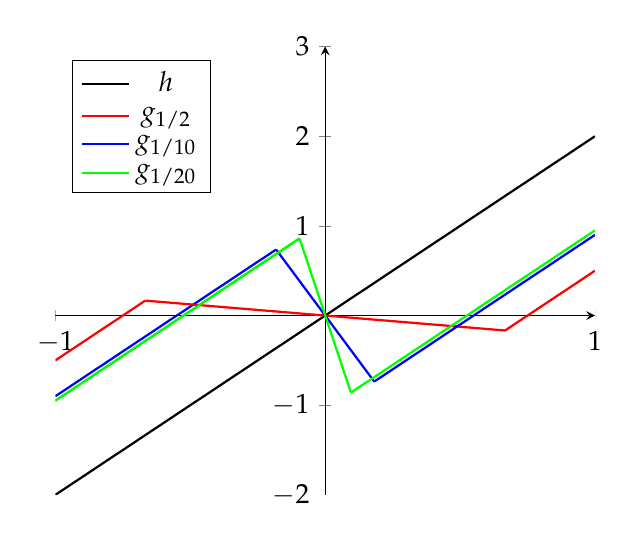
\begin{tikzpicture}\begin{axis}[axis lines = middle, 
xmin=-1,xmax=1,
ymin=-2,ymax=3,     
xtick={-1,0,1},     
ytick={-2,-1,1,2,3},
legend pos= north west,]


\addplot [domain=-1:1,samples=100,color=black,thick] ({x}, {2*x});
\addplot [domain=-1:-0.666,samples=100,color=red,thick] ({x}, {2*x+1+0.5});
\addplot [domain=-1:-0.1818,samples=100,color=blue,thick] ({x}, {2*x+1+0.1});
\addplot [domain=-1:-0.095,samples=100,color=green,thick] ({x}, {2*x+1+0.05});
\addplot [domain=-0.666:0.666,samples=100,color=red,thick] ({x}, {-0.25*x});
\addplot [domain=0.666:1,samples=100,color=red,thick] ({x}, {2*x+1-2.5});
\addplot [domain=-0.1818:0.1818,samples=100,color=blue,thick] ({x}, {-4.05*x});
\addplot [domain=0.1818:1,samples=100,color=blue,thick] ({x}, {2*x+1-2.1});
\addplot [domain=-1:-0.095,samples=100,color=green,thick] ({x}, {2*x+1+0.05});
\addplot [domain=-0.095:0.095,samples=100,color=green,thick] ({x}, {-9.025*x});
\addplot [domain=0.095:1,samples=100,color=green,thick] ({x}, {2*x+1-2.05});


\addlegendentry{$ h $} 
\addlegendentry{$ g_{1/2}$}
\addlegendentry{$ g_{1/10}$} 
\addlegendentry{$ g_{1/20}$}

\end{axis}\end{tikzpicture}\end{center}

Now observe that
\begin{align*}
\int_{-1}^{0}g_{t}(x)\mathrm{d}x & =\int_{-1}^{\frac{-2t}{1+t}}(2x+1+t)\mathrm{d}x+\int_{\frac{-2t}{1+t}}^{0}-\frac{(t-1)^{2}}{2t}x\mathrm{d}x\\
 & =(x^{2}+x+tx)|_{-1}^{\frac{-2t}{1+t}}+\left(\frac{-(t-1)^{2}}{4t}x^{2}\right)|_{\frac{-2t}{1+t}}^{0}\\
 & =\left(\frac{2t}{1+t}\right)^{2}+\left(\frac{-2t}{1+t}\right)+t\left(\frac{-2t}{1+t}\right)-\left(1-1-t\right)+\frac{(t-1)^{2}}{4t}\left(\frac{2t}{1+t}\right)^{2}\\
 & =\left(\frac{(t-1)^{2}}{4t}+1\right)\left(\frac{2t}{1+t}\right)^{2}+(1+t)\left(\frac{-2t}{1+t}\right)+t\\
 & =\frac{(t+1)^{2}}{4t}\frac{4t^{2}}{(1+t)^{2}}-t\\
 & =t-t\\
 & =0.
\end{align*}
Therefore $g_{t}\in\mathcal{Y}$ for all $t\in(0,1]$. Moreover, by
construction we have 
\[
\|g_{t}-h\|_{\infty}=1+t
\]
for all $t\in(0,1]$. This implies $d(h,\mathcal{Y})\leq1$. 

\hfill

\textbf{Step 2: }We claim that there does not exist a $g\in\mathcal{Y}$
such that $\|g-h\|_{\infty}=1$. Indeed, assume for a contradiction
there does exist a $g\in\mathcal{Y}$ such that $\|g-h\|_{\infty}=1$.
Choose such a $g\in\mathcal{Y}$. We may assume that $g$ is real-valued:
if $g$ is not real-valued, then we pass to its real-valued part $u$
and as argued above we obtain $u\in\mathcal{Y}$ and 
\begin{align*}
1 & =\|g-h\|_{\infty}\\
 & =\|u-h\|_{\infty}\\
 & \geq1.
\end{align*}

Since $g$ is real-valued and $\|g-h\|_{\infty}=1$, we have
\[
2x-1\leq g(x)\leq2x+1
\]
for all $x\in[-1,1]$. Since $g$ is continous, we cannot have 
\[
g(x)=\begin{cases}
2x+1 & \text{for all }x\in(-1,0)\\
2x-1 & \text{for all }x\in(0,1).
\end{cases}
\]
Assume $g(x)\neq2x-1$ on the interval $(0,1)$. Choose $c\in(0,1)$
such that $g(c)\neq2c-1$. Since $g$ is continuous and since $g(c)>2c-1$,
there exists $\varepsilon>0$ and $\delta>0$ such that 
\[
g(x)>2x-1+\varepsilon
\]
for all $x\in(c-\delta,c+\delta)$. Choose such $\varepsilon$ and
$\delta$ so that $(c-\delta,c+\delta)\subset(0,1)$. Then
\begin{align*}
0 & =\int_{0}^{1}g(x)\mathrm{d}x\\
 & =\int_{0}^{1}g(x)\mathrm{d}x+\int_{c-\delta}^{c+\delta}g(x)\mathrm{d}x+\int_{c+\delta}^{1}g(x)\mathrm{d}x\\
 & >\int_{0}^{c-\delta}(2x-1)\mathrm{d}x+\int_{c-\delta}^{c+\delta}(2x-1+\varepsilon)\mathrm{d}x+\int_{c+\delta}^{1}(2x-1)\mathrm{d}x\\
 & =\int_{0}^{1}(2x-1)\mathrm{d}x+\int_{c-\delta}^{c+\delta}\varepsilon\mathrm{d}x\\
 & =(x^{2}-x)|_{0}^{1}+\varepsilon x|_{c-\delta}^{c+\delta}\\
 & =2\varepsilon\delta\\
 & >0
\end{align*}
gives us a contradiction.

~~~Thus $g(x)\neq2x+1$ on the interval $(-1,0)$. Choose $c\in(-1,0)$
such that $g(c)\neq2c+1$. Then by a similar argument as above, we
have
\begin{align*}
0 & =\int_{-1}^{0}g(x)\mathrm{d}x\\
 & <\int_{-1}^{0}(2x+1)\mathrm{d}x-\int_{c-\delta}^{c+\delta}\varepsilon\mathrm{d}x\\
 & =-2\varepsilon\delta\\
 & <0,
\end{align*}
which also gives us a contradiction. Therefore there does not exist
a $g\in\mathcal{Y}$ such that $\|g-h\|_{\infty}=1$. \end{proof}

\section*{Problem 6}

\begin{defn}\label{defn} Let $\mathcal{X}$ be a normed linear space.
For a set $A\subseteq\mathcal{X}$ we define $A^{\perp}$ to be the
subset of $\mathcal{X}^{*}$ consisting of all $\ell\in\mathcal{X}^{*}$
such that $\ell(a)=0$ for all $a\in A$. Similarly, for a set $M\subseteq\mathcal{X}^{*}$
we define $M_{\perp}$ to be the subset of $\mathcal{X}$ consisting
of all vectors $x\in\mathcal{X}$ such that $\ell(x)=0$ for all $\ell\in M$.
\end{defn}

\begin{prop}\label{propclosedsubspacesperpantiperp} Let $\mathcal{X}$
be a normed linear space, let $A$ be a subset of $\mathcal{X}$,
and let $M$ be a subset of $\mathcal{X}^{*}$. Then $A^{\perp}$
and $M_{\perp}$ are closed subspaces of $\mathcal{X}^{*}$ and $\mathcal{X}$
respectively. \end{prop}

\begin{proof} Let $x\in\mathcal{X}$. Define $\widehat{x}\colon\mathcal{X}^{*}\to\mathbb{C}$
by
\[
\widehat{x}(\ell)=\ell(x)
\]
for all $\ell\in\mathcal{X}^{*}$. We claim that $\widehat{x}$ is
a bounded linear functional. To see that $\widehat{x}$ is linear,
let $\ell,\ell'\in\mathcal{X}^{*}$ and let $\lambda,\lambda'\in\mathbb{C}$.
Then
\begin{align*}
\widehat{x}(\lambda\ell+\lambda'\ell') & =(\lambda\ell+\lambda'\ell')(x)\\
 & =\lambda\ell(x)+\lambda'\ell'(x)\\
 & =\lambda\widehat{x}(\ell)+\lambda'\widehat{x}(\ell').
\end{align*}
To see that $\widehat{x}$ is bounded, let $\ell\in\mathcal{X}^{*}$.
Then
\begin{align*}
|\widehat{x}(\ell)| & =|\ell(x)|\\
 & \leq\|x\|\|\ell\|.
\end{align*}
Therefore $\widehat{x}$ is a bounded linear functional. In particular
$\text{ker}\widehat{x}$ is a closed subspace. Thus
\[
A^{\perp}=\bigcap_{a\in A}\text{ker}\widehat{a}\quad\text{and}\quad M_{\perp}=\bigcap_{\ell\in M}\text{ker}\ell
\]
are closed subspaces since an arbitrary intersection of closed subspaces
is a closed subspace. \end{proof}

\begin{prop}\label{prop} Let $\mathcal{X}$ be a normed linear space,
let $A$ be a subset of $\mathcal{X}$, and let $M$ be a subset of
$\mathcal{X}^{*}$. Then $\overline{\text{span}}(A)\subseteq(A^{\perp})_{\perp}$
and $\overline{\text{span}}(M)\subseteq(M_{\perp})^{\perp}$. \end{prop}

\begin{proof} Proposition~(\ref{propclosedsubspacesperpantiperp})
implies $(A^{\perp})_{\perp}$ and $(M_{\perp})^{\perp}$ are closed
subspace. Thus, it suffices to show
\[
\text{span}(A)\subseteq(A^{\perp})_{\perp}\quad\text{and}\quad\text{span}(M)\subseteq(M_{\perp})^{\perp}.
\]
~~~First we show the former. Let $\lambda_{1}a_{1}+\cdots+\lambda_{n}a_{n}\in\text{span}(A)$
and let $\ell\in A^{\perp}$. Then since $\ell(a)=0$ for all $a\in A$,
we have
\begin{align*}
\ell(\lambda_{1}a_{1}+\cdots+\lambda_{n}a_{n}) & =\lambda_{1}\ell(a_{1})+\cdots+\lambda_{n}\ell(a_{n})\\
 & =\lambda_{1}\cdot0+\cdots+\lambda_{n}\cdot0\\
 & =0.
\end{align*}
Since $\ell$ was arbitrary, this implies $\lambda_{1}a_{1}+\cdots+\lambda_{n}a_{n}\in(A^{\perp})_{\perp}$,
and hence $\text{span}(A)\subseteq(A^{\perp})_{\perp}$. 

~~~Now we show the latter. Let $\lambda_{1}\ell_{1}+\cdots+\lambda_{n}\ell_{n}\in\text{span}(M)$
and let $x\in M_{\perp}$. Then since $\ell(x)=0$ for all $\ell\in M$,
we have
\begin{align*}
(\lambda_{1}\ell_{1}+\cdots+\lambda_{n}\ell_{n})(x) & =\lambda_{1}\ell_{1}(x)+\cdots+\lambda_{n}\ell_{n}(x)\\
 & =\lambda_{1}\cdot0+\cdots+\lambda_{n}\cdot0\\
 & =0.
\end{align*}
Since $x$ was arbitrary, this implies $\lambda_{1}\ell_{1}+\cdots+\lambda_{n}\ell_{n}\in(M_{\perp})^{\perp}$,
and hence $\text{span}(M)\subseteq(M_{\perp})^{\perp}$. \end{proof}

\section*{Problem 7}

\begin{prop}\label{prop} $(\ell^{1})^{*}$ is isometrically isomorphic
to $\ell^{\infty}$. \end{prop}

\begin{proof} For each $n\in\mathbb{N}$, let $e^{n}$ denote the
sequence with entry $1$ in the $n$th component and entry $0$ everywhere
else. Define $\Phi\colon(\ell^{1})^{*}\to\ell^{\infty}$ by
\[
\Phi(\psi)=(\psi(e^{n}))
\]
for all $\psi\in(\ell^{1})^{*}$. Note that for any $\psi\in(\ell^{1})^{*}$,
we have $|(\psi(e^{n}))|\leq\|\psi\|$, and therefore $(\psi(e^{n}))\in\ell^{\infty}$.
We claim that $\|\psi\|=\|\Phi(\psi)\|_{\infty}$. Indeed,
\begin{align*}
\|\Phi(\psi)\|_{\infty} & =\sup\{|\psi(e^{n})|\mid n\in\mathbb{N}\}\\
 & \leq\sup\left\{ \left|\psi\left(\sum_{n=1}^{\infty}a_{n}e^{n}\right)\right|\mid\sum_{n=1}^{\infty}|a_{n}|\leq1\right\} \\
 & =\|\psi\|.
\end{align*}
To prove the reverse inequality assume for a contradiction that $\|\psi\|>\|\Phi(\psi)\|_{\infty}$.
Choose $\varepsilon>0$ and $\sum_{n=1}^{\infty}a_{n}e^{n}\in\ell^{1}$
such that $\sum_{n=1}^{\infty}|a_{n}|\leq1$ and
\begin{equation}
\left|\psi\left(\sum_{n=1}^{\infty}a_{n}e^{n}\right)\right|>\|\Phi(\psi)\|_{\infty}+\varepsilon.\label{eq:strictineq1}
\end{equation}
Choose $N\in\mathbb{N}$ such that $\sum_{n=N}^{\infty}|a_{n}|<\varepsilon/\|\psi\|$
(we can find such an $N$ since $\sum_{n=1}^{\infty}|a_{n}|<\infty$).
Then
\begin{align*}
\left|\psi\left(\sum_{n=1}^{\infty}a_{n}e^{n}\right)\right| & =\left|\psi\left(\sum_{n=1}^{N}a_{n}e^{n}+\sum_{n=N+1}^{\infty}a_{n}e^{n}\right)\right|\\
 & =\left|\psi\left(\sum_{n=1}^{N}a_{n}e^{n}\right)+\psi\left(\sum_{n=N+1}^{\infty}a_{n}e^{n}\right)\right|\\
 & =\left|\sum_{n=1}^{N}a_{n}\psi(e^{n})+\psi\left(\sum_{n=N+1}^{\infty}a_{n}e^{n}\right)\right|\\
 & \leq\left|\sum_{n=1}^{N}a_{n}\psi(e^{n})\right|+\left|\psi\left(\sum_{n=N+1}^{\infty}a_{n}e^{n}\right)\right|\\
 & \leq\sum_{n=1}^{N}|a_{n}||\psi(e^{n})|+\|\psi\|\sum_{n=N+1}^{\infty}|a_{n}|\\
 & <\|\Phi(\psi)\|_{\infty}\sum_{n=1}^{N}|a_{n}|+\|\psi\|\cdot\frac{\varepsilon}{\|\psi\|}\\
 & \leq\|\Phi(\psi)\|_{\infty}+\varepsilon.
\end{align*}
This contradicts (\ref{eq:strictneq1}).

~~~Next we show $\Phi$ is linear. Let $\varphi,\psi\in(\ell^{1})^{*}$
and let $\lambda,\mu\in\mathbb{C}$. Then
\begin{align*}
\Phi(\lambda\varphi+\mu\psi) & =((\lambda\varphi+\mu\psi)(e^{n}))\\
 & =\lambda(\varphi(e^{n}))+\mu(\psi(e^{n}))\\
 & =\lambda\Phi(\varphi)+\mu\Phi(\psi).
\end{align*}

Therefore $\Phi$ is an isometric embedding. 

~~~Now show that $\Phi$ is surjective, and hence an isometric
isomorphism. Let $(a_{n})\in\ell^{\infty}$, let $M=\sup\{|a_{n}|\}$,
and let $E=\text{span}\{e^{n}\mid n\in\mathbb{N}\}$. Define $\varphi\colon E\to\mathbb{C}$
to be the unique linear map such that
\[
\varphi(e^{n})=a_{n}
\]
 for all $n\in\mathbb{N}$. Let $x=x_{n_{1}}e^{n_{1}}+\cdots+x_{n_{k}}e^{n_{k}}\in E$
such that $|x_{n_{1}}|+\cdots+|x_{n_{k}}|\leq1$. Then
\begin{align*}
|\varphi(x_{n_{1}}e^{n_{1}}+\cdots+x_{n_{k}}e^{n_{k}})| & =|x_{n_{1}}\varphi(e^{n_{1}})+\cdots+x_{n_{k}}\varphi(e^{n_{k}})|\\
 & =|x_{n_{1}}a_{n_{1}}+\cdots+x_{n_{k}}a_{n_{k}}|\\
 & \leq|x_{n_{1}}||a_{n_{1}}|+\cdots+|x_{n_{k}}||a_{n_{k}}|\\
 & \leq|x_{n_{1}}|M+\cdots+|x_{n_{k}}||M\\
 & =(|x_{n_{1}}|+\cdots+|x_{n_{k}}||)M\\
 & \leq M
\end{align*}
It follows that $\varphi$ is bounded. By the Hahn-Banach Theorem,
there exists a bounded linear functional $\widetilde{\varphi}$ defined
on all of $\ell^{1}$ such that $\widetilde{\varphi}|_{E}=\varphi$
and $\|\widetilde{\varphi}\|=\|\varphi\|$. Choose such a $\widetilde{\varphi}\in(\ell^{1})^{*}$.
Then clearly $\Phi(\widetilde{\varphi})=(a_{n})$. Therefore $\Phi$
is surjective, and hence an isometric isomorphism. \end{proof}

\section*{Appendix}

\subsection*{Problem 1}

\begin{prop}\label{propsuplinearpositive} Let $A$ be a non-emtpy
set of real numbers which is bounded above and let $\lambda$ be any
non-negative real number. Then
\begin{equation}
\sup(\lambda A)=\lambda\sup(A).\label{eq:sup}
\end{equation}

\end{prop}

\begin{proof} If $\lambda=0$, then (\ref{eq:sup}) is obvious, so
assume $\lambda>0$. Let $\alpha$ denote $\sup(A)$. Choose any element
in $\lambda A$, say $\lambda a$ where $a\in A$. Then since $a\leq\alpha$
and $\lambda$ is non-negative, we have $\lambda a\leq\lambda\alpha$.
This implies
\[
\sup(\lambda A)\leq\lambda\sup(A).
\]
For the reverse direction, observe that
\begin{align*}
\sup(A) & =\sup(\lambda^{-1}\lambda A)\\
 & \leq\lambda^{-1}\sup(\lambda A),
\end{align*}
and this implies 
\[
\sup(\lambda A)\geq\lambda\sup(A).
\]

\end{proof}

\begin{prop}\label{propsuplinearpositive2} Let $A$ and $B$ be non-empty
sets of non-negative real numbers both of which are bounded above.
Then
\begin{equation}
\sup(A+B)=\sup(A)+\sup(B).\label{eq:sup-1}
\end{equation}

\end{prop}

\begin{proof} Let $\alpha$ denote $\sup(A)$, let $\beta$ denote
$\sup(B)$, and let $a+b$ be an arbitrary element in $A+B$. Then
$a\leq\alpha$ and $b\leq\beta$ implies $a+b\leq\alpha+\beta$. Therefore
\begin{equation}
\sup(A+B)\leq\sup(A)+\sup(B).\label{eq:ineqsupadd}
\end{equation}
To show the reverse inequality, we assume (for a contradiction) that
the inequality (\ref{eq:ineqsupadd}) is strict
\[
\sup(A+B)<\sup(A)+\sup(B).
\]
Choose $\varepsilon>0$ such that 
\begin{equation}
\sup(A+B)<\sup(A)+\sup(B)-\varepsilon.\label{supstrictin}
\end{equation}
Choose $a\in A$ and $b\in B$ such that $a>\alpha-\varepsilon/2$
and $b>\beta-\varepsilon/2$. Then
\begin{align*}
a+b & >\alpha-\frac{\varepsilon}{2}+\beta-\frac{\varepsilon}{2}\\
 & =\alpha+\beta-\varepsilon.
\end{align*}
But this contradicts (\ref{supstrictin}). Therefore 
\[
\sup(A+B)\geq\sup(A)+\sup(B).
\]

\end{proof}
\end{document}
